 \providecommand{\main}{../../..}
\documentclass[\main/main.tex]{subfiles}
\begin{document}
\subsection{Esercizio 1}
Dato il seguente problema di PL:

\begin{figure}
  \begin{align*}
    \min z = x_1 -2x_2   \\
    x_1 + 4x_2 & \leq 32 \\
    x_1 - 2x_2 & \leq 2  \\
    x_1 + x_2  & \geq 5  \\
    -x_1 + x_2 & \leq 3  \\
    x_1, x_2   & \geq 0
  \end{align*}
  \caption{Esercizio 1}
\end{figure}

\begin{enumerate}
  \item Si disegni la regione ammissibile e si evidenzi il vertice ottimo per via grafica, riportando il valore di z e di tutte le variabili del modello, comprese quelle di scarto.
  \item Si ricavi per via grafica per quali valori di $b_1$, ora pari a $32$, la \textbf{composizione} della base ottima non cambia.
  \item Si risolva mediante gli scarti complementari il duale del problema.
\end{enumerate}

\subsection{Soluzione esercizio 1}

\subsubsection*{Identifico soluzione ottima}

\begin{figure}
  \begin{subfigure}{0.49\textwidth}
    \dddgraph{x_1}{x_2}{0}{12}{0}{7}{-10}{x + 4*y <= 32&&  x - 2*y <= 2&&  x + y >= 5&&  -x + y <= 3}{x -2*x}
    \caption{Il vertice ottimo ha coordinate $\bmx = \rnd{4,7}$}
  \end{subfigure}
  \begin{subfigure}{0.49\textwidth}
    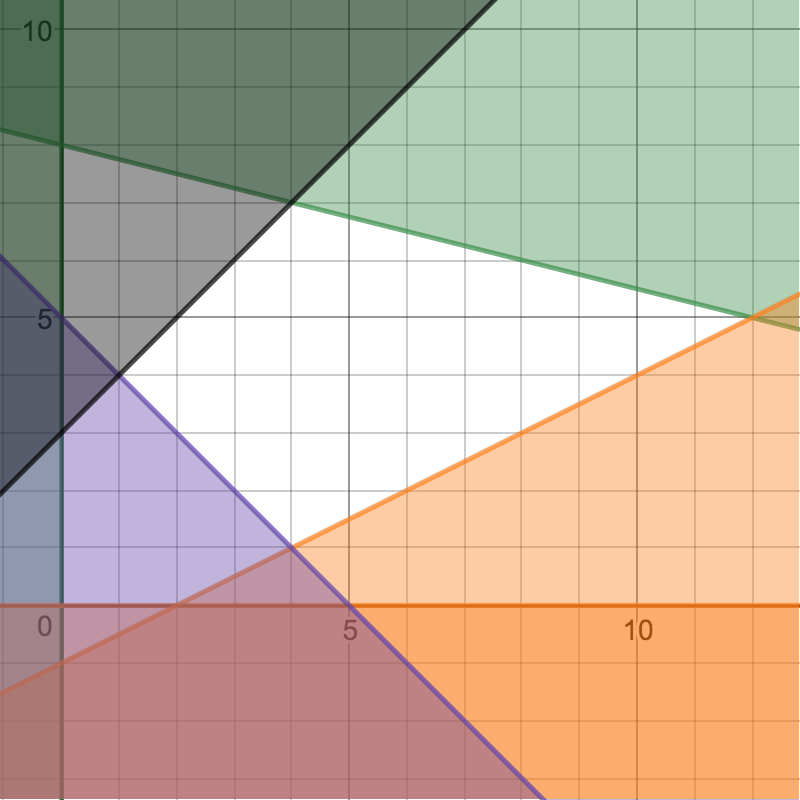
\includegraphics[width=0.9\textwidth]{2014_11_17}
    \caption{Regione di ammissibilità del problema}
  \end{subfigure}
  \caption{Vertice ottimo del problema di minimo}
\end{figure}

\subsubsection*{Riporto variabili}

\begin{align*}
  z = -10, \quad
  x_1 = 4, \quad
  x_2 = 7, \quad
  s_1 = 0, \quad
  s_2 = 8, \quad
  s_3 = 6, \quad
  s_4 = 0
\end{align*}
\subsubsection*{Analisi di sensitività}
Riducendo il valore di $b_1$ sino a $17$ la base ottima si sposta sino a $(1,4)$. Non esiste un valore massimo per $b_1$ che modifica la base ottima.
\begin{figure}
  \begin{subfigure}{0.49\textwidth}
    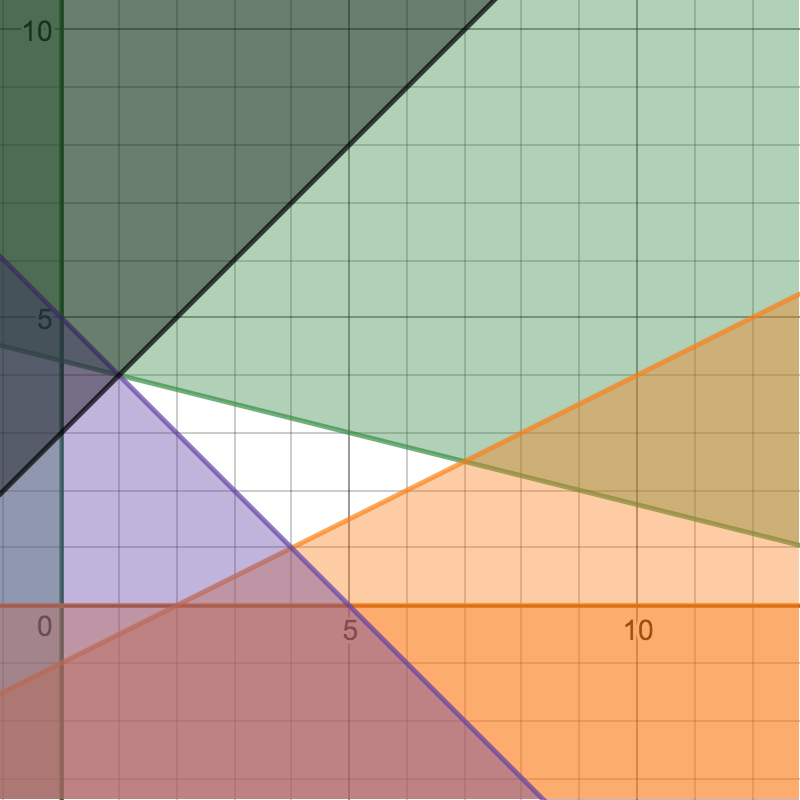
\includegraphics[width=0.9\textwidth]{2014_11_17_1}
    \caption{$b=17$}
  \end{subfigure}
  \begin{subfigure}{0.49\textwidth}
    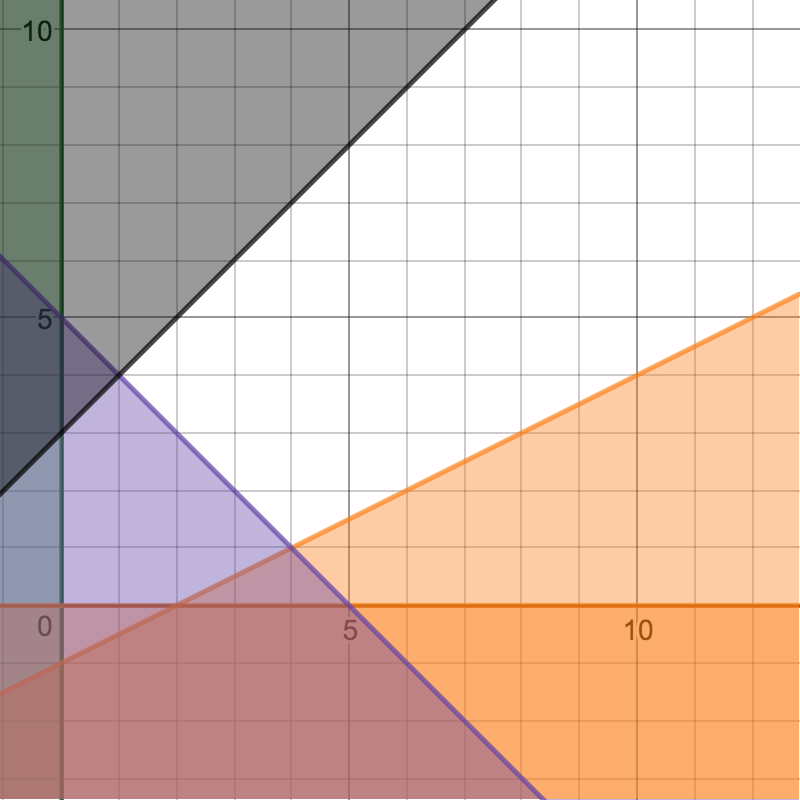
\includegraphics[width=0.9\textwidth]{2014_11_17_2}
    \caption{$b=+\infty$}
  \end{subfigure}
  \caption{Analisi di sensitività}
\end{figure}

\subsubsection*{Costruisco problema duale}
\begin{align*}
  \max z_D = 32y_1 + 2y_2 + 5y_3 + 3y_4 \\
  y_1 + y_2 + y_3 -y_4  & \leq 1        \\
  4y_1 -2y_2 + y_3 -y_4 & \leq -2       \\
  y_1, y_2, y_4         & \leq 0        \\
  y_3                   & \geq 0
\end{align*}
\subsubsection*{Scarti complementari}
\[
  \begin{cases}
    x_1(y_1 + y_2 + y_3 -y_4  - 1 )=0 \\
    x_2(4y_1 -2y_2 + y_3 +y_4 + 2)=0  \\
    y_1(x_1 + 4x_2 -32)=0             \\
    y_2(x_1 - 2x_2 -2 )=0             \\
    y_3(x_1 + x_2  -5 )=0             \\
    y_4(-x_1 + x_2 -3 )=0             \\
  \end{cases}
  \Rightarrow
  \begin{cases}
    y_1  -y_4  - 1=0 \\
    4y_1 +y_4 + 2=0  \\
    y_2=0            \\
    y_3=0            \\
  \end{cases}
  \Rightarrow
  \begin{cases}
    y_4=-\frac{6}{5} \\
    y_1=-\frac{1}{5} \\
    y_2=0            \\
    y_3=0            \\
  \end{cases}
\]
La soluzione ottima del problema duale coincide con la soluzione ottima del problema primale: $z = z_D = -10$.
\end{document}